%% ============================================================================
%%
%%  Master's thesis
%% 
%%  Author: FORNAVN EFTERNAVN
%%
%%  Chapter 1: Coffee
%% ============================================================================

\chapter{BBN physics and cosmology}
\label{chap:theory}

To understand the process of Big Bang nucleosynthesis, we must examine the intersection between cosmology, thermodynamics, particle, nuclear and statistical physics. Though this might seem daunting, it turns out that the unique conditions during this epoch allow for extensive simplifications of this otherwise monumental task. Throughout this thesis we use $\hbar=c=k_B=1$.



% ~~~~~~~~~~~~~~~~~~~~~~~~~~~~~~~~~~~~~~~~~~~~~~~~~~~~~~~~~~~~~~~~~~~~~~~~~~~~~
% SECTION
% ~~~~~~~~~~~~~~~~~~~~~~~~~~~~~~~~~~~~~~~~~~~~~~~~~~~~~~~~~~~~~~~~~~~~~~~~~~~~~
\section{Determining background parameters}
\label{sec:Background}
Nuclear processes in the early universe are governed by two main parameters, the density of the baryons and their temperature. The density will decrease as the universe expands, so we need to track this expansion using the scale factor $a$, which is a simple dimensionless scalar, proportional to the expansion of the universe. In the early universe, baryons were in thermodynamic equilibrium with the photons, so to track their temperature we just need to track the temperature of the photons, $T$. 


\subsection{Scale factor}
\label{ssec:cosmology}

BBN takes place after inflation while the universe is still radiation-dominated. The expansion can be described by the Friedman equation, which can be simplified with the reasonable approximation, that both curvature and the cosmological constant are zero \cite[{(4.29)}]{Ryden}. 
\begin{align}
    H^2=\left(\frac{\dot{a}}{a}\right)^2=\frac{8\pi G}{3}\rho_{tot},
    \label{Friedman}
\end{align}
with H being the Hubble parameter, G the gravitational constant and $\rho_{tot}$ referring to the total energy density of photons, leptons and baryons,
\begin{align}
    \rho_{tot}=\rho_{\gamma}+\rho_{\nu}+(\rho_{e^-}+\rho_{e^+})+\rho_{b}.
\end{align}
\eqref{Friedman} can be rearranged as a differential equation explicitly describing the time evolution of the scale factor.
\begin{align}
    \diff{a}{t}=a\sqrt{\frac{8\pi G}{3}\rho_{tot}(T,a)}
    \label{eq:dadt}
\end{align}

\subsection{Temperature}
To find an expression for the temperature evolution, we utilize energy conservation. We can consider the neutrinos as decoupled from the other particles during BBN, and so the photon temperature will be determined by the remaining components. Since the universe at this point is very much homogeneous and isotropic, we utilize the fluid equation for adiabatic expansion \cite[{(4.44)}]{Ryden}, to describe the time evolution of the density of coupled components.
\begin{align}
    \dot{\rho_{set}}+3\frac{\dot{a}}{a}(\rho_{set} + P_{set})=0
\end{align}
With $\rho_{set}$ being the density of none-decoupled components and $P_{set}$ being their pressures.
\begin{align}
    \rho_{set}=\rho_{\gamma}+(\rho_{e^-}+\rho_{e^+})+\rho_{b}
    \eqsep P_{set}=P_{\gamma}+(P_{e^-}+P_{e^+})+P_{b}
\end{align}
Using the chain rule $\dot{\rho}=\dot{T}\idiff{\rho}{T}$, we can then set up a differential equation describing the time evolution of the photon temperature. 
\begin{align}
    \diff{T}{t}=-3\frac{\dot{a}}{a}\frac{\rho_{set}(T,a) + P_{set}(T,a)}{\diff{\rho_{set}(T,a)}{T}}
    \label{eq:dTdt}
\end{align}

\subsection{Additional parameters}
For this code, the only necessary cosmological parameters are the scale factor and temperature, but other BBN codes often track different parameters. Most BBN codes are based on the original code by Wagoner described in section \ref{sec:BBN_history}. These don't track the scale factor, but instead use the quantity $h$.
\begin{align}
    h=M_u\frac{n_{b}}{T^3_9},
\end{align}
with $M_u$ being atomic mass units, $n_b$ the baryon number density, and  $T_9$ the temperature in $10^9$ Kelvin. This quantity was useful since it stays approximately constant throughout BBN, while being easy to directly convert to baryon density. However, with modern computers this numerical simplicity is inconsequential, and as such it is more instructive to track the scale factor.
The electron chemical potential was also tracked by the Wagoner code and its successors. The main effect of this is ensuring a non-zero electron density after $e^-$ $e^+$ annihilation. We can easily set this to 0, as the impact will be 3 orders of magnitude lower than the already minuscule impact of the baryon density.

\textcolor{orange}{Neutrino temperature?}


\section{Energy densities and pressure of different particles}
To solve \cref{eq:dTdt,eq:dadt}, we need to know the density and pressure of the components of the early universe. To do this we first need to derive the general equations for the energy and pressure of a collection of relativistic particles, before going over each component.

\subsection{Relativistic gasses}
In the very early universe most particles were in thermal equilibrium, and can thus be described by the rules of statistical physics. Here the average number of particles in a given state is governed by the Fermi-Dirac distribution for fermions, and the Bose-Einstein distribution for bosons.
\begin{align}
    \bar{n}_{FD}=\frac{1}{e^{(E-\mu)/T}+1} \eqsep   \bar{n}_{BE}=\frac{1}{e^{(E-\mu)/T}-1},
    \label[equation]{fermionboson}
\end{align}
with $E$ being the total energy of each particle in the state and $\mu$ the chemical potential. Using the average number of particles in a given state, the total number density can be found by integrating over all possible momentum states. 
\begin{align}
    n(T)=\frac{g}{(2\pi)^3}\int_{0}^{\infty}\bar{n}(p,T)dp^3=\frac{g}{2\pi^2}\int_{0}^{\infty}\bar{n}(p,T) p^2 dp,
    \label[equation]{numberdensity}
\end{align}
with g being the degeneracy parameter, describing the number of distinct states with a given momentum. We can similarly find an expression for the energy density by multiplying the integrand by the relativistic energy $E^2=m^2+p^2$.
\begin{align}
    \rho(T)=\frac{g}{2\pi^2}\int_{0}^{\infty}\bar{n}(p,T)\sqrt{m^2+p^2} p^2 dp
    \label[equation]{energydensity}
\end{align}
The pressure can be similarly determined by identifying the pressure exerted by a single relativistic particle with some momentum $p$.
Pressure is defined as the force exerted per unit area. Consider a relativistic particle confined to a sphere of radius $r$. Whenever it collides with the surface, it will exert a force proportional to the change in momentum. 
\begin{align}
    F=\diff{p}{t}=\frac{\Delta p }{\Delta t}\eqsep
    \Delta p = 2p \cos \theta,
    \label{eq:pressureF}
\end{align}
with $\theta$ being the incident angle. 

The time between collisions can be deduced based on the distance traveled.
\begin{align}
    \Delta t = \frac{L}{\mathrm{v}}=L\frac{\sqrt{m^2+p^2}}{p},
    \label{eq:pressureDeltat}
\end{align}
with distance between collisions $L$, and velocity $\mathrm{v}$. Where we have used $p=m\gamma \mathrm{v}$ and $E=m\gamma$, to relate velocity to momentum.

Next, consider the triangle created by the center of the sphere and two consecutive collision points. Using the law of cosines we can determine $L$,
\begin{align}
    r^2=L^2+r^2+2L r \cos \theta \Rightarrow
    L = 2r \cos \theta.
    \label{eq:pressureL}
\end{align}
Combining \cref{eq:pressureF,eq:pressureDeltat,eq:pressureL}, we can determine the force and pressure exerted on the sphere by each particle. 
\begin{align}
    F = \frac{p^2}{r\sqrt{m^2+p^2}} \eqsep P = \frac{p^2}{4\pi r^3\sqrt{m^2+p^2}}
\end{align}
Generalizing this for any volume, we get a quantity analogous to the energy of a single particle,
\begin{align}
    PV=\frac{p^2}{3\sqrt{m^2+p^2}} .
    \label[equation]{Pcontribution}
\end{align}
Integrating with $PV$ will give us the total pressure, just as integrating with energy gives the energy density.
\begin{align}
    P(T)=\frac{g}{6\pi^2}\int_{0}^{\infty}\bar{n}(p,T)\frac{p^4}{\sqrt{m^2+p^2}}dp
    \label[equation]{pressure}
\end{align}
Additionally, we see that the pressure of an ultra-relativistic gas follows a simple relation.
\begin{align}
    P(T)=\frac{\rho(T)}{3} \quad (\text{for } m\ll p)
    \label[equation]{Prho3}
\end{align}
With this we can determine the density and pressure of each component, starting with the photons.

\subsection{Photons}
Photons are massless bosons with 2 distinct polarizations for each momentum state. With $g=2$, we use \eqref{energydensity} to determine the energy density. 
\begin{align}
    \rho_\gamma(T)=\int_{0}^{\infty} \frac{p^3}{\pi^2}\frac{1}{e^{p/T}-1}dp =  \frac{T^4}{\pi^2}\int_{0}^{\infty}\frac{u^3}{e^{u}-1}du
\end{align}
By changing the integration variable to $u=p/T$, the integral becomes a well-known representation of the Riemann Zeta function \cite[\href{https://dlmf.nist.gov/25.5.E1}{(25.5.1)}]{NIST:DLMF}, with the following solution
\begin{align}
    \rho_\gamma(T)=\frac{T^4}{\pi^2}\Gamma(4)\zeta(4)=\frac{\pi^2}{15}T^4
    \label[equation]{rhogamma}.
\end{align}
From this we can easily determine the temperature derivative and pressure.
\begin{align}
    \diff{\rho_\gamma(T)}{T}=\frac{4}{15}\pi^2T^3 \eqsep P_\gamma(T)=\frac{\rho_\gamma(T)}{3}
\end{align}
The same procedure can be used to determine the number density,
\begin{align}
    n_\gamma(T)=\frac{T^3}{\pi^2}\int_{0}^{\infty}\frac{u^2}{e^{u}-1}du=\frac{T^3}{\pi^2}\Gamma(3)\zeta(3)
    \label{eq:ngamma}.
\end{align}



\subsection{Neutrinos}
\label{sec:rhoNeutrino}
For neutrinos $g=2N_\nu$, to account for the different species and their antiparticles.
\begin{align}
    \rho_\nu(T_\nu)=N_\nu\int_{0}^{\infty} \frac{p^3}{\pi^2}\frac{1}{e^{p/T_\nu}+1}dp =  N_\nu\frac{T_\nu^4}{\pi^2}\int_{0}^{\infty}\frac{u^3}{e^{u}+1}du
\end{align}
This is another integral representation of the Riemann Zeta function \cite[\href{https://dlmf.nist.gov/25.5.E3}{(25.5.3)}]{NIST:DLMF}.
\begin{align}
    \rho_\nu(T_\nu)=N_\nu\frac{T_\nu^4}{\pi^2}\Gamma(4)\zeta(4)(1-2^3)=N_\nu\frac{7}{8}\frac{\pi^2}{15}T_\nu^4.
    \label[equation]{rhonu}
\end{align}
This relation only holds if the neutrinos follow a Fermi-Dirac distribution, which is not exactly true at later times, since their gradual decoupling from the other components introduces non-thermal distortions to their energy distribution. However, if the neutrinos are completely decoupled, their energy can instead be described using only the scale factor 
\begin{align}
    \rho_\nu(t)=\frac{\rho_\nu(T_i)}{a(t)^4},
    \label[equation]{realrhonu}
\end{align}
with $T_i$ being the initial temperature where neutrinos are still in thermal equilibrium and $a=1$. This has the added advantage of eliminating the need for tracking the neutrino temperature. The major downside is that this does not take into account the small energy transfer from e${^+}$ e${^-}$-annihilation due to incomplete decoupling of neutrinos. To compensate we can replace the number of neutrinos $N_\nu=3$, with an effective neutrino number $N_\nu^\text{eff}=3.045$, (\textcite{de_Salas_2016}), corresponding to the predicted increase in energy. The impact of incomplete neutrino decoupling is discussed further in section \ref{sec:decoupling}.




\subsection{Electrons and positrons}


Since electrons and positrons have mass, solving for their density and pressure is a lot more intricate than for the massless particles.
\begin{align}
    \rho_\pm(T)=\frac{1}{\pi^2}\int_{0}^{\infty}\frac{\sqrt{m^2+p^2}}{e^{(E\pm\mu)/T}+1}p^2 dp
    \label[equation]{rhoe}
\end{align}
\begin{align}
    P_\pm(T)=\frac{1}{3\pi^2}\int_{0}^{\infty}\frac{1}{e^{(E\pm\mu)/T}+1}\frac{p^4}{\sqrt{m^2+p^2}} dp
\end{align}
Inspired by the derivation of Chandrasekhar \cite{Chandrasekhar}, we will solve these integrals by using the rapidity $\theta$.
\begin{align}
    \sinh \theta = \frac{p}{m}\eqsep \cosh \theta = \frac{E}{m}
    \label[equation]{rapiditet}
\end{align}
After a simple change of variable we get a much nicer form of the integrals.
\begin{align}
    \rho_\pm(T)=\frac{m^4}{\pi^2}\int_{0}^{\infty}\frac{\sinh^2 \theta \cosh^2\theta}{e^{(m \cosh\theta\pm\mu)/T}+1} d\theta
    \label[equation]{rhoet}
\end{align}
\begin{align}
    P_\pm(T)=\frac{m^4}{3\pi^2}\int_{0}^{\infty}\frac{\sinh^4 \theta}{e^{(m \cosh\theta\pm\mu)/T}+1} d\theta
    \label[equation]{Pet}
\end{align}
Next, we start by considering the geometric series.
\begin{align}
    \frac{1}{1+x}=\sum_{n=0}^{\infty}(-1)^n x^n \eqsep \text{for  }  \left|x\right|<1
\end{align}
Multiplying both sides by x grants us a very useful expansion,
\begin{align}
    \frac{1}{x^{-1}+1}=\sum_{n=1}^{\infty}(-1)^{n+1} x^n \eqsep \text{for  }  \left|x\right|<1.
\end{align}
Before and during BBN, $(E\pm\mu)/T $ will be strictly positive, enabling $x=e^{-(E\pm\mu)/T}$.
\begin{align}
    \frac{1}{e^{(m \cosh\theta\pm\mu)/T}+1}=\sum_{n=1}^{n=\infty} (-1)^{n+1} e^{-n\frac{m }{T}\cosh\theta}e^{\mp n\frac{\mu}{T}}
    \label{eq:electronseries}
\end{align}
The chemical potential does not depend on the rapidity, allowing us to get the combined pressure of both electrons and positrons, using $e^{-\phi}+e^{\phi}=2\cosh\phi$
\begin{align}
    P_e(T)=P_-+P_+=\frac{2m^4}{3\pi^2}\sum_{n=1}^{n=\infty} (-1)^{n+1} \cosh{\left(n\frac{\mu}{T}\right)}  \int_{0}^{\infty}e^{-n\frac{m }{T}\cosh\theta}\sinh^4 \theta d\theta
\end{align}
These terms are integral representations of modified Bessel functions \cite[\href{https://dlmf.nist.gov/10.32.E8}{(10.32.8)}]{NIST:DLMF}.
\begin{align}
    \int_{0}^{\infty}e^{-z\cosh\theta}\sinh^4 \theta d\theta=4\frac{\Gamma(2+\frac{1}{2})}{\sqrt{\pi}z^2}K_2\left(z\right)=3z^{-2}K_2\left(z\right)
\end{align}
With $z=n\frac{m }{T}$, we can get the total pressure expressed as a sum of modified Bessel functions.
\begin{align}
    P_e(T)=\frac{2m^2}{\pi^2} T^2 \sum_{n=1}^{n=\infty} \frac{(-1)^{n+1}}{n^{2}} \cosh{\left(n\frac{\mu}{T}\right)}   K_2\left(n\frac{m }{T}\right)
    \label{eq:Pelectron}
\end{align}
The energy density can be found in the same way, by first utilizing the identity $cosh^2=sinh^2+1$, to get the energy density in terms of $\sinh\theta$.
\begin{align}
    \rho_e(T)=\rho_-+\rho_+=\frac{2m^4}{\pi^2}\sum_{n=1}^{n=\infty} (-1)^{n+1} \cosh{\left(n\frac{\mu}{T}\right)}  \int_{0}^{\infty}e^{-n\frac{m }{T}\cosh\theta}\left(\sinh^4\theta +\sinh^2\theta\right) d\theta
\end{align}
The $\sinh^4$ term is clearly the same as for the pressure up to a factor of 3. Comparing this to the results for massless particles, this term can be interpreted as the thermal energy of the electron gas. The second term also corresponds to a modified Bessel function, though of first rather than second-order \cite[\href{https://dlmf.nist.gov/10.32.E8}{(10.32.8)}]{NIST:DLMF}. Combined this grants us the sum describing the total energy density of electrons and positrons.
\begin{align}
    \rho_e(T)=\frac{2m^2}{\pi^2} T^2 \sum_{n=1}^{n=\infty} \frac{(-1)^{n+1}}{n^{2}} \cosh{\left(n\frac{\mu}{T}\right)}  \left( 3 K_2\left(n\frac{m }{T}\right) + n\frac{m }{T} K_1\left(n\frac{m }{T}\right) \right)
    \label{eq:rhoelectron}
\end{align}
Using recursion relations for the modified Bessel functions \cite[\href{https://dlmf.nist.gov/10.29.E1}{(10.29.1)}]{NIST:DLMF}, we see that this is equivalent to the expression used in other BBN codes \cite{Kawano}.
\begin{align}
3K_{2}(z)+z K_{1}(z)=3\frac{z}{4}[K_{3}(z)-K_{1}(z)]+z K_{1}(z)=\frac{z}{4}[3K_{3}(z)+K_{1}(z)]
\end{align}
\begin{align}
    \rho_e(T)=\frac{m^3}{2\pi^2} T \sum_{n=1}^{n=\infty} \frac{(-1)^{n+1}}{n} \cosh{\left(n\frac{\mu}{T}\right)}  \left( 3 K_3\left(n\frac{m }{T}\right) + K_1\left(n\frac{m }{T}\right) \right)
\end{align}
As mentioned many older BBN codes track the parameter $\phi_e=\frac{\mu}{T}$, but this is unnecessary, as the electron density after $e^-$ $e^+$ annihilation is three orders of magnitude lower than the already negligible contribution of the baryons. So for the remaining calculation we set $\mu = 0$.

Finding the temperature derivative of the electron energy density can also be achieved using the recursion relations for Bessel functions \cite[\href{https://dlmf.nist.gov/10.29.E2}{(10.29.2)}]{NIST:DLMF}.
\begin{align}
    \diff{}{z} \frac{1}{z}[3K_{3}(z)+K_{1}(z)]&=-3[z^{-2} K_{3}(z)+z^{-1} K_{2}(z)+ 3z^{-2} K_{3}(z)]-z^{-1} K_{2}\\
    &=-12 z^{-2} K_{3}(z)-4z^{-1} K_{2}(z)\\
    &=-\frac{1}{z}[2K_{4}(z)-2K_{2}(z)+4 K_{2}(z)]\\
    &=-\frac{2}{z}[K_{4}(z)+K_{2}(z)]
\end{align}
With this we can determine the temperature derivative.
\begin{align}
    \diff{\rho_e(T)}{z}=-\frac{m^3}{\pi^2} T \sum_{n=1}^{n=\infty} \frac{(-1)^{n+1}}{n}  \left(K_4\left(n\frac{m }{T}\right) + K_2\left(n\frac{m }{T}\right) \right)\\
    \diff{\rho_e(T)}{T}=\frac{m^4}{\pi^2} \frac{1}{T} \sum_{n=1}^{n=\infty} (-1)^{n+1}   \left(K_4\left(n\frac{m }{T}\right) + K_2\left(n\frac{m }{T}\right) \right)
\end{align}


\subsection{Baryons}





The temperatures at which BBN takes place are too low for baryon pair production. Therefore, the number density of baryons can be solely determined by the scale factor and some known density. 
\begin{align}
    n_b(a)=\frac{a_0^3}{a^3}n_{b}(a_0),
\end{align}
with $a_0$ being the scale factor at a time when we know the corresponding number density $n_{b}(a_0)$. To determine baryon density $n_{b}(a_0)$, we use the baryon photon/ratio $\eta$, and the photon number density given by \cref{eq:ngamma}, 
\begin{align}
    n_b=n_\gamma(T) \eta \eqsep n_\gamma(T)=\frac{T^3}{\pi^2}\Gamma(3)\zeta(3).
\end{align}
From the CMB we can measure the value of $\eta$ during recombination, but unlike baryons the number of photons does not remain unchanged from the start of BBN until recombination. The only significant source of photons is the annihilation of the electron-positron pairs. We can account for this using conservation of entropy. For a given species we define the entropy density \cite[(3.91)]{kolbturner},
\begin{align}
    s=\frac{\rho+P}{T}.
\end{align}
Setting $a=1$ at the start of our BBN calculations, we get a relation between the total entropy before and after annihilation.
\begin{align}
     s_{\gamma}(T_{CMB})a_{CMB}^3= s_e(T_{i})+s_{\gamma}(T_{i})
    \label{eq:entropycon}
\end{align}
The photon number density is directly proportional to entropy density, both scaling with $T^3$. This allows us to restate \eqref{eq:entropycon} only in terms of the initial entropy density.
\begin{align}
    n_{\gamma}(T_{CMB})a_{CMB}^3 = \frac{n_\gamma(T_{i})}{s_{\gamma}(T_{i})}\left(s_e(T_{i})+s_{\gamma}(T_{i})\right)
\end{align}
From this we get the baryon density as a function of the initial photon and electron density and pressure.
\begin{align}
    n_b(a_{CMB}){a_{CMB}^3}=n_\gamma(T_{i}) \left(\frac{s_e(T_{i})+s_{\gamma}(T_{i})}{s_{\gamma}(T_{i})}\right)\eta
\end{align}
\begin{align}
    n_b(a)=\frac{1}{a^3}n_\gamma(T_{i}) \left(1+\frac{\rho_e(T_{i})+P_{e}(T_{i})}{\rho_{\gamma}(T_{i})+P_{\gamma}(T_{i})}\right)\eta
    \label{n_b}
\end{align}
with $T_i$ being the initial temperature. Finally, to get the energy density we simply need to sum over all different nuclei. 
\begin{align}
    \rho_b(a)=n_b(a)\sum_{i}^{}Y_i m_i
    \label{rhob}
\end{align}
For each isotope, $m_i$ is the mass, and $Y_i$ is the ratio between the number of nuclei and the total number of nucleons. $Y_i$ is often defined as $Y_i=X_i/A_i$, with $X_i$ being the mass fraction, and $A_i$ the atomic weight \cite{Wagoner69}. The difference in per nucleon mass of different isotopes, causes these two definitions to have a relative difference of $10^{-5}$, which can be safely neglected when looking at total mass. Furthermore, we can approximate that all baryons have the same mass as a lone proton which reduces \eqref{rhob} to $\rho_b(a) \approx n_b(a)m_p$. 

Employing the chain rule we can write the temperature derivative as 
\begin{align}
    \diff{\rho_b(a)}{T} = -3\rho_b(a)\frac{1}{a}\diff{a}{T}.
\end{align}
Since the universe is radiation-dominated we can relate the scale factor and temperature as $a\propto T^{-1}$. This is not precise enough to be used for the background as a whole especially during $e^-$ $e^+$-annihilation, but it will suffice for this already minor term, allowing us to evaluate the derivative
\begin{align}
    \diff{\rho_b(a)}{T} = 3\rho_b(a)T^{-1}.
    \label{drhob}
\end{align}
The baryon pressure can be found using the ideal gas law.
\begin{align}
    P_b(a)= n_b(a)T\sum_{i}^{}Y_i
\end{align}
Unlike that of the relativistic particles, the baryon pressure is several orders of magnitude lower than the density. Since the baryon density is already comparatively low, the pressure will be completely negligible.

%Baryon density impact on abundance
%array([1.0000975 , 1.00000049, 1.0000059 , 1.00000433, 1.00000195,
%0.99999851, 1.00000364, 0.99999819, 1.00006305, 0.99999216,
%1.00000415, 1.00025283, 1.00000866, 0.99994947, 1.00009333,
%1.00027059, 0.99999412, 0.99999102, 0.99998706, 1.00063686,
%1.00036322, 0.99998709, 0.99997431, 1.00077921, 1.00039927,
%0.99998262])


%invm=A**2/m_Nucs
%def altrho_bY_cgs(y):
%return eta_ini*n_gamma_ini/y[1]**3*gcm3/np.dot(y[n_bparams:6+n_bparams],invm[:6])
%plt.figure()
%plt.plot(soltime/timeunit,np.array([a_cache(soltime[i])**3*rho_bY_cgs(np.array([T_cache(soltime[i]),a_cache(soltime[i])]+list(solY[:,i]))) for i in range(len(soltime))])/np.array([a_cache(soltime[i])**3*altrho_bY_cgs(np.array([T_cache(soltime[i]),a_cache(soltime[i])]+list(solY[:,i]))) for i in range(len(soltime))]),label='Normal density')

%
%
% ~~~~~~~~~~
% SUBSECTION
% ~~~~~~~~~~
\section{Nuclear reactions}
\label{sec:nucleartheory}

All relevant nuclear reactions involve at most 6 different nuclei. Generally we can write these reactions as
\begin{align}
    N_i X_i + N_j X_j + N_k X_k \leftrightharpoons N_n X_n + N_m X_m + N_l X_l ,
\end{align}
where $N_i$ is the number of nuclei $X_i$, that enter the reaction. 
The change in abundance $Y_i$ of any nuclei is given by the sum of all reactions that create or destroy it.\footnote{\url{https://pynucastro.github.io/pynucastro/rate_types.html}}
\begin{align}
    \diff{Y_i}{t}=\sum_{\lambda_i}\frac{N_i}{n_b}\left(\lambda_{n m l \rightarrow i j k} \frac{Y_n^{N_n}Y_m^{N_m}Y_l^{N_l}}{N_n!N_m!N_l!}n_b^{(N_n+N_m+N_l)}-\lambda_{i j k \rightarrow n m l}\frac{Y_i^{N_i}Y_j^{N_j}Y_l^{N_k}}{N_i!N_j!N_k!}n_b^{(N_i+N_j+N_k)}\right)
    \label{dYdt}
\end{align}
With $\lambda$ being the reaction rate, and $n_b$ being the baryon number density. The reaction rate $\lambda(T)$ only depends on the kinetic energy of the baryons and by extension the photon temperature. $n_b(a)$ only depends on the scale factor as shown in \eqref{n_b}. 

From \eqref{dYdt} we can quite easily determine the partial derivatives required for the construction of a Jacobian. 
\begin{align}
    \pdiff{}{Y_j}\diff{Y_i}{t}&=-\sum_{\lambda_{ij\rightarrow}}N_i N_j\lambda_{i j k \rightarrow n m l}\frac{Y_i^{N_i}Y_j^{N_j-1}Y_l^{N_k}}{N_i!N_j!N_k!}n_b^{(N_i+N_j+N_k-1)}\label{eq:jacterms1}\\
    \pdiff{}{Y_n}\diff{Y_i}{t}&=\sum_{\lambda_{n \rightarrow i }}N_i N_n\lambda_{n m l \rightarrow i j k} \frac{Y_n^{N_n-1}Y_m^{N_m}Y_l^{N_l}}{N_n!N_m!N_l!}n_b^{(N_n+N_m+N_l-1)}
    \label{eq:jacterms2}
\end{align}


\subsection[Proton to neutron rate]{Proton $\leftrightharpoons$ neutron rate}
At $T>10^{10}$K any created nuclei will be instantly destroyed by high energy photons. This leaves only the conversion between neutrons and positrons, which is governed by the following reactions
\begin{align}
    n &\leftrightarrow p+e^-+\bar{\nu}_e\\
    n+e^+ &\leftrightarrow p+\bar{\nu}_e\\
    n+\nu_e &\leftrightarrow p+e^-
\end{align}
The final reaction $p\leftrightarrow n+e^++\nu_e$ is not possible, as it would violate energy conservation, which is apparent if one considers the reaction from the rest frame of the proton. For most other rates, we can measure $\lambda$ experimentally for the forward rate $Q>0$, and use detailed balance to estimate the corresponding reverse rate. The conditions required for maintaining nuclear statistical equilibrium between neutrons and protons cannot be achieved experimentally, and the rate therefore must be determined theoretically. This involves evaluating several integrals, which depend on both electron and neutrino density, in addition to the temperature and scale factor. Several corrections must also be made to account for the radiative, zero-temperature, corrections, finite nucleon mass corrections, finite temperature radiative corrections, weak-magnetism, and QED plasma effects\cite{PRIMAT}. 
The final result mainly depends on temperature and experimentally determined mean neutron lifetime, $\tau_n$. Since it isn't affected by the later reactions, it is sensible to just fit the result as a function of temperature and mean lifetime. 
For the default network in APODORA, the rate is described by the parameterization given in appendix C of \textcite{Serpico_2004}.
\begin{align}
    \lambda_{n\rightarrow p}&=\frac{1}{\tau_n}e^{-q_{np}/z}\sum_{i=0}^{13}a_i z^{-i}\quad\eqsep 0.01\leq T/\text{MeV} \leq 10 \\
    \lambda_{p\rightarrow n}&=
\begin{cases}
    \frac{1}{\tau_n}e^{-q_{pn}\cdot z}\sum_{i=0}^{10}b_i z^{-i}&,\quad\ \ 0.1\leq T/\text{MeV} \leq 10\\
        0&,\quad 0.01\leq T/\text{MeV} \leq 0.1
\end{cases}
\end{align}
with the fitted parameters being the constants $a_i$ and $b_i$ as well as $q_{np}$ and $q_{pn}$. 

%\chapter{Nuclear abundances}

\section{Initial conditions}
The initial value of the scale factor can be set as $a=1$. This leaves the temperature and time which are directly linked. As none of the earlier equations have any explicit time dependence, it is more useful to choose an initial temperature, and then determine the initial time based on this.

\subsection{Initial temperature}
When performing BBN calculations, it is most sensible to choose an initial temperature, and from it, determine all other initial conditions. The chosen temperature should be sufficiently high, so that all particles are in thermal equilibrium. Most BBN codes use $T=27\times10^9$K as the initial temperature. Higher temperatures could be used, but this is unnecessary and will often lead to numerical instabilities, which will be covered in \cref{chap:BBNcode,sec:Accuracy}.

\subsection{Initial time}
\label{sec:t_ini}
Though none of the equations describing BBN have any explicit time dependence, it is still nice to know the age of the universe when it takes place. This can be achieved by integrating equation \eqref{eq:dTdt}, with $T=\infty$ at $t=0$.
\begin{align}
    %\diff{T}{t}=\mp\sqrt{24\pi G\rho_{tot}}\frac{\rho_{set}(T,a) + P_{set}(T,a)}{\diff{\rho_{set}(T,a)}{T}}\\
    \int_{0}^{t_i}dt=\int_{\infty}^{T_i}\left(\diff{T}{t}\right)^{-1}dT=-\int_{\infty}^{T_i}(24\pi G\rho_{tot})^{-1/2}\frac{\diff{\rho_{set}(T)}{T}}{\rho_{set}(T) + P_{set}(T)}dT
    \label{eq:ti_integral}
\end{align}
For high temperatures we can assume that the electrons are completely relativistic. Based on the result for neutrinos \eqref{rhonu}, we know that the energy of a massless fermion differs from that of a boson by a factor of $7/8$. Accounting for the g factors, we get $\rho_e=7/4 \rho_\gamma$. At temperatures above 2 MeV the relativistic approximation deviates by less than 1\%, see figure \ref{fig:rhoegammaT}.
\begin{figure}[ht]
    %\centering
    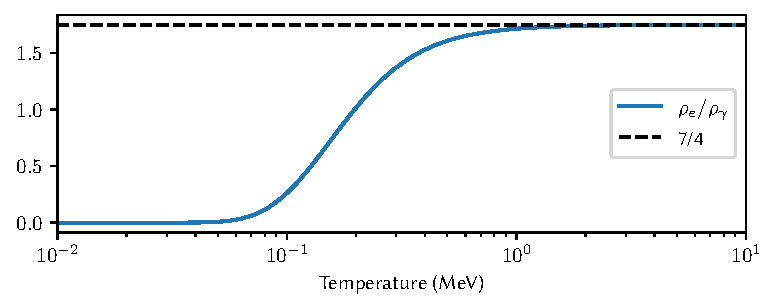
\includegraphics[width=5.1in]{figures/rhoegammaT.pdf}
    \caption{Exact ratio of the electron-positron energy to the photon energy}
    \label{fig:rhoegammaT}
\end{figure}

At these temperatures we can safely ignore the baryon contribution, which combined with \eqref{Prho3}, allows us to calculate the non-decoupled terms.
\begin{align}
    \frac{\diff{\rho_{set}(T)}{T}}{\rho_{set}(T) + P_{set}(T)}=\frac{3}{4}\frac{1}{\rho_{set}(T)}\diff{\rho_{set}(T)}{T}=3T^{-1}
\end{align}
For the total energy we simply add the contributions of all components, excluding baryons,
\begin{align}
    \rho_{tot}=\rho_\gamma+(2+3)\frac{7}{8}\rho_\gamma=\frac{43}{8}\rho_\gamma
\end{align}
Inserting into \eqref{eq:ti_integral}, we get the initial time,
\begin{align}
    t_i&=3(24\pi G\frac{43}{8}\frac{\pi^2}{15})^{-1/2}\int_{\infty}^{T_i}T^{-3}dT\\
    t_i&=\frac{3}{2}( \frac{43}{5}G\pi^3)^{-1/2}T_i^{-2}
    \label{eq:t_ini}
\end{align}
This relation is valid at all times before decoupling, and remains approximately true at later times, as shown on figure \ref{fig:Temperature}.
\begin{figure}[ht]
    %\centering
    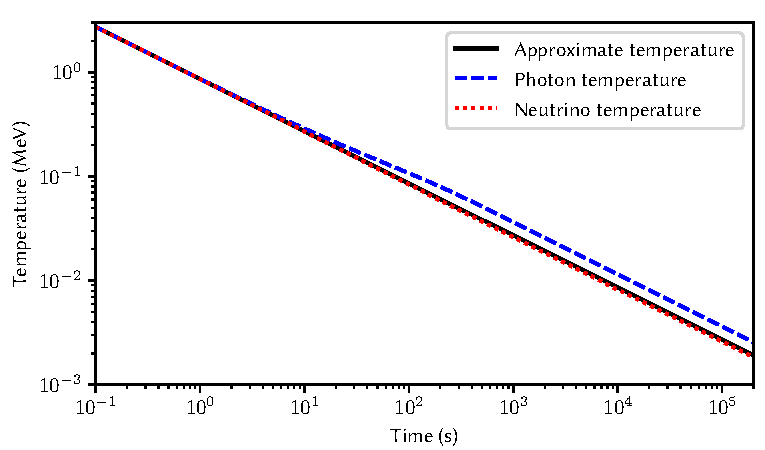
\includegraphics[width=5.1in]{figures/Temperature.pdf}
    \caption{The temperature of photons and neutrinos during the time period of BBN, as well as the approximate temperature given by \eqref{eq:t_ini}}
    \label{fig:Temperature}
\end{figure}

To get a sense of scale for this result we can rewrite it in units of $10^9K$ and seconds.
\begin{align}
    T_9=( 43 \frac{4}{3}\pi\frac{a_r}{c^2}G)^{-1/4}t^{-1/2}=9.97t^{-1/2},
    \label{eq:T9_ini}
\end{align}
with $a_r$ being the radiation constant, related to the Stefan–Boltzmann constant by $a=\frac{4}{c}\sigma$. 
Using this we can justify the omission of particles heavier than electrons. The lightest of these are the muon and pion, which both have masses above 100 MeV. Significant pair creation will occur at $T_9 \geq 10^3$, corresponding to $t\approx10^4$. As such they will have no significant impact on the initial time. 

\subsection{Initial time in existing literature}
We note that \eqref{eq:T9_ini} differs significantly from the expression derived by Wagoner\cite{Wagoner67},
\begin{align}
    T_9=(12\pi\frac{a_r}{c^2}G)^{1/4}t^{-1/2}=10.4t^{-1/2},
\end{align}
The analytical expression is wrong, but the numerical result is correct. A simple error which probably was the result of a small mistake when transcribing the notes used for the paper. Unfortunately, this expression has been reproduced in several later BBN codes such as \texttt{NUC123}\cite{Kawano} and \textsc{AlterBBN}\cite{AlterBBN}. Though Kawano reproduced the equation in the documentation, in the actual \texttt{NUC123} code he used the numerical result and as such the code itself had no errors. In \textsc{AlterBBN} they used natural units, and so couldn't use the numerical value, leading to the error affecting the code. Additionally, they also confused the Stefan–Boltzmann and radiation constants leading to an additional error. Examining the code, one can see that their value is wrong by 14 orders of magnitude. %which they seemly discovered and erroneously corrected by doing an additional conversion from $\hbar/GeV$ to seconds. This brings the final value to a few mi
Since it doesn't impact final abundances, this error was only very recently discovered, with the first correction being released in 2021 by Sharpe \cite{sharpe2021big},
\begin{align}
    T_9=(48\pi\frac{a_r}{c^2}G)^{-1/4}t^{-1/2}=10.4t^{-1/2},
\end{align}
However this still differs from \eqref{eq:T9_ini}. This is due to the fact that the original derivation was performed by Wagoner in 1967, a decade before the discovery of the tau and corresponding neutrino. Though later projects correctly added the additional neutrino flavor when calculating the neutrino energy, the impact it has on the initial time had been overlooked before this thesis. 



%Warning test\fxwarning{This is a warning!}






